\chapter{Преобразование случайных векторов}


\section*{Введение}
Пусть $X$ и $Y$ --- случайные величины, и $a$, $b$ и $c$ --- числа.

Для математического ожидания справедливо свойство линейности:
\begin{equation}
    \expectation{a \cdot X + b \cdot Y + c}
    = a \cdot \expectation{X} + b \cdot \expectation{Y} + c
\end{equation}
а для дисперсии справедливо равенство:
\begin{equation}
    \variance{a \cdot X + b \cdot Y + c}
    = a^2 \cdot \variance{X} + b^2 \cdot \variance{Y} + 2 a b \cdot \covariance{X}{Y},
\end{equation}
где
\begin{multline}
    \label{10:covariance}
    \covariance{X}{Y}
    = \expectation{\left ( X - \expectation{X} \right ) \left ( Y - \expectation{Y} \right )} = \\
    %
    = \expectation{ X Y - \expectation{X} Y - X \expectation{Y} - \expectation{X} \expectation{Y}} = \\
    %
    = \expectation{XY} - \expectation{X} \expectation{Y} - \expectation{X} \expectation{Y} + \expectation{X} \expectation{Y} = \\
    %
    = \expectation{XY} - \expectation{X} \expectation{Y}.
\end{multline}
Для \textbf{независимых} случайных величин:
\begin{equation}
    \covariance{X}{Y}
    = \expectation{\left ( X - \expectation{X} \right ) \left ( Y - \expectation{Y} \right )}
    = \left ( \expectation{X} - \expectation{X} \right ) \left ( \expectation{Y} - \expectation{Y} \right )
    = 0 \cdot 0
    = 0 .
\end{equation}


\section*{Задача 18.437}

Случайные величины $X$ и $Y$ независимы и имеют следующие характеристики: $m_X = 1$, $m_Y = 2$, $\sigma_X = 1$, $\sigma_Y = 2$.
Вычислить математические ожидания случайных величин:
\begin{enumerate}
    \item $U = X^2 + 2 Y^2 - XY - 4X + Y + 4$,
    \item $V = (X + Y - 1)^2$
\end{enumerate}

\subsection*{Решение:}
\begin{enumerate}
    \item По свойству линейности математического ожидания:
    \begin{multline}
        \label{10:437:U}
        \expectation{U}
        = \expectation{X^2 + 2 Y^2 - XY - 4X + Y + 4} = \\
        = \expectation{X^2} + 2 \expectation{Y^2} - \expectation{XY} - 4 \expectation{X} + \expectation{Y} + \expectation{4}
    \end{multline}

    Для вычисления вторых начальных моментов используем известное соотношение для дисперсии:
    \begin{gather}
        \variance{X} = \expectation{X^2} - \left ( \expectation{X} \right )^2 , \\
        \variance{X} + \left ( \expectation{X} \right )^2 = \expectation{X^2} \label{10:437:X_2}.
    \end{gather}
    и
    \begin{equation}
        \label{10:437:Y_2}
        \expectation{Y^2} = \variance{Y} + \left ( \expectation{Y} \right )^2.
    \end{equation}

    По условию задачи величины $X$ и $Y$ \textbf{независимы}, поэтому:
    \begin{gather}
        \expectation{XY} = \expectation{X} \cdot \expectation{Y}
    \end{gather}

    Подставляя полученные выражения в равенство \eqref{10:437:U}, получим:
    \begin{multline}
        \expectation{U}
        = \variance{X} + \left ( \expectation{X} \right )^2 + 2 \left ( \variance{Y} + \left ( \expectation{Y} \right )^2 \right ) - \expectation{X} \cdot \expectation{Y} - 4 \expectation{X} + \expectation{Y} + \expectation{4} = \\
        = \sigma_X^2 + m_X^2 + 2 \left ( \sigma_Y^2 + m_Y^2 \right ) - m_X m_Y - 4 m_X + m_Y + 4 = \\
        = 1^2 + 1^2 + 2 \left ( 2^2 + 2^2 \right ) - 1 \cdot 2 - 4 \cdot 1 + 2 + 4 = 18
        .
    \end{multline}

    \item Заметим, что величина $V$ является квадратом выражения, и требуется найти второй начальный момент:
    \begin{equation}
        \label{10:437:expectation}
        \expectation{V} = \expectation{\left ( X + Y - 1 \right )^2} = \variance{X + Y - 1} + \left ( \expectation{X + Y - 1} \right )^2 ,
    \end{equation}
    где в последнем равенстве использовалось выражение для второго момента через дисперсию и квадрат математического ожидания, как ранее, в выражениях \eqref{10:437:X_2}
    и \eqref{10:437:Y_2}.
    По свойствам дисперсии:
    \begin{equation}
        \label{10:437:variance}
        \variance{X + Y - 1} = \variance{X} + \variance{Y} + 2 \covariance{X}{Y}
    \end{equation}
    Ковариация величин $X$ и $Y$ из равенства \eqref{10:covariance}:
    \begin{equation}
        \covariance{X}{Y} = \expectation{XY} - \expectation{X} \expectation{Y}.
    \end{equation}
    В силу \textbf{независимости} величин $X$ и $Y$:
    \begin{equation}
        \covariance{X}{Y} = 0 ,
    \end{equation}
    а выражение для дисперсии \eqref{10:437:variance} принимает вид:
    \begin{equation}
        \variance{X + Y - 1} = \variance{X} + \variance{Y} .
    \end{equation}
    и выражение \eqref{10:437:expectation}:
    \begin{multline}
        \expectation{V}
        = \variance{X} + \variance{Y} + \left ( \expectation{X} + \expectation{Y} - 1 \right )^2 = \\
        %
        = \sigma_X^2 + \sigma_Y^2 + \left ( m_X + m_Y - 1 \right )^2
        = 1^2
        + 2^2 + \left ( 1 + 2 - 1 \right )^2
        = 9.
    \end{multline}
\end{enumerate}

\subsection*{Ответ}
\begin{enumerate}
    \item $\expectation{U} = 18$ ,
    \item $\expectation{V} = 9$.
\end{enumerate}


\section*{Задача 18.438}

Случайная точка $\left ( X, Y \right )$ характеризуется центром рассеивания $(-1, 1)$ и ковариационной матрицей
$\begin{pmatrix}
     3  & -2 \\
     -2 & 4
\end{pmatrix}$.
Найти математическое ожидание и дисперсию случайной величины $Z = 2 X - 4 Y + 3$.

\subsection*{Решение:}

Центр рассеивания:
\begin{equation}
    \begin{pmatrix}
        -1 \\
        1
    \end{pmatrix}
    =
    \begin{pmatrix}
        \expectation{X} \\
        \expectation{Y}
    \end{pmatrix}
    .
\end{equation}

Ковариационная матрица
\begin{equation}
    \begin{pmatrix}
        3  & -2 \\
        -2 & 4
    \end{pmatrix}
    =
    \begin{pmatrix}
        \variance{X}      & \covariance{X}{Y} \\
        \covariance{X}{Y} & \variance{Y}
    \end{pmatrix}
    .
\end{equation}

В силу линейности математического ожидания:
\begin{equation}
    \expectation{Z}
    = \expectation{2X - 4 Y + 3}
    = 2 \expectation{X} - 4 \expectation{Y} + 3
    = 2 \cdot (-1) - 4 \cdot 1 + 3
    = -3
    .
\end{equation}
и по свойствам дисперсии:
\begin{multline}
    \variance{Z}
    = \variance{2 X - 4 Y + 3}
    = \variance{2 X + (-4) Y + 3} = \\
    %
    = 2^2 \cdot \variance{X} + (-4)^2 \cdot \variance{Y} + 2 \cdot 2 \cdot (-4) \cdot \covariance{X}{Y} = \\
    %
    = 4 \cdot 3 + 16 \cdot 4 - 16 \cdot (-2)
    = 12 + 16 \cdot 6
    = 12 + 96
    = 108.
\end{multline}

\subsection*{Ответ}
$\expectation{Z} = -3$, $\variance{Z} = 108$.


\section*{Задача 18.443}

Случайная величина $X$ дискретного типа распределена по закону, определяемому таблицей:

\begin{tabular}{|c|c|c|c|}
    \hline
    $x_i$ & -1            & 0             & 1             \\
    \hline
    $p_i$ & $\frac{1}{6}$ & $\frac{1}{3}$ & $\frac{1}{2}$ \\
    \hline
\end{tabular}

Найти коэффициент корреляции между $X$ и $X^2$.

\subsection*{Решение:}

По определению коэффициент корреляции $\rho$:
\begin{equation}
    \rho = \frac{\covariance{X}{X^2}}{\sqrt{\variance{X} \variance{X^2}}}
\end{equation}

Представим ковариацию с помощью моментов:
\begin{equation}
    \covariance{X}{X^2}
    = \expectation{X \cdot X^2} - \expectation{X} \cdot \expectation{X^2}
    = \expectation{X^3} - \expectation{X} \cdot \expectation{X^2}
\end{equation}

Заметим, что у величины $X$ нечетные начальные моменты ($k=1,2,3,...$):
\begin{equation}
    \expectation{X^{2k-1}} = \sum_{i=1}^3 x_i^{2k-1} \cdot p_i = (-1)^{2k-1} \cdot \frac{1}{6} + 0^{2k-1} \cdot \frac{1}{3} + 1^{2k-1} \cdot \frac{1}{2} = - \frac{1}{6} + \frac{1}{2} = \frac{1}{3} ,
\end{equation}
и чётные начальные моменты ($k=1,2,3,...$):
\begin{equation}
    \expectation{X^{2k}} = \sum_{i=1}^3 x_i^{2k} \cdot p_i = (-1)^{2k} \cdot \frac{1}{6} + 0^{2k} \cdot \frac{1}{3} + 1^{2k} \cdot \frac{1}{2} = \frac{1}{6} + \frac{1}{2} = \frac{2}{3} .
\end{equation}

Таким образом, ковариация:
\begin{equation}
    \covariance{X}{X^2} = \frac{1}{3} - \frac{1}{3} \cdot \frac{2}{3} = \frac{3}{9} - \frac{2}{9} = \frac{1}{9} .
\end{equation}

Вычислим дисперсии:
\begin{gather}
    \variance{X} = \expectation{X^2} - \left ( \expectation{X} \right )^2 = \frac{2}{3} - \left ( \frac{1}{3} \right )^2 = \frac{6}{9} - \frac{1}{9} = \frac{5}{9} , \\
    \variance{X^2} = \expectation{X^4} - \left ( \expectation{X^2} \right )^2 = \frac{2}{3} - \left ( \frac{2}{3} \right )^2 = \frac{6}{9} - \frac{4}{9} = \frac{2}{9}.
\end{gather}

Таким образом, коэффициент корреляции:
\begin{equation}
    \rho = \frac{\frac{1}{9}}{\sqrt{\frac{5}{9} \cdot \frac{2}{9}}} = \frac{\frac{1}{9}}{\frac{1}{9} \sqrt{10}} = \frac{1}{\sqrt{10}} .
\end{equation}

\subsection*{Ответ:}
$\frac{1}{\sqrt{10}}$.

\section*{Задача 18.515}

Случайные величины $X$ и $Y$ независимы и подчиняются одному и тому же индикаторному распределению $B(1,p)$. Описать законы распределения случайных величин
$Z = X + Y$ и $V = X Y$.
\subsection*{Решение:}
Величина $X$ подчиняется индикаторному распределению $B(1,p)$ означает, что $X$ принимает значение 1 с веростноятью $p$ и 0 с вероятностью $1-p$:

\begin{tabular}{|c|c|}
    \hline
    $X$ & $P$   \\
    \hline
    0   & $1-p$ \\
    \hline
    1   & $p$   \\
    \hline
\end{tabular}

Составим таблицы значения для вероятностей и значений величин $Z$ и $V$:

\begin{tabular}{|c|c|c|c|c|}
    \hline
    $X$ & $Y$ & $P$                 & $Z$ & $V$ \\
    \hline
    0   & 0   & $(1-p) \cdot (1-p)$ & 0   & 0   \\
    \hline
    1   & 0   & $p \cdot (1-p)$     & 1   & 0   \\
    \hline
    0   & 1   & $(1-p) \cdot p$     & 1   & 0   \\
    \hline
    1   & 1   & $p \cdot p$         & 2   & 1   \\
    \hline
\end{tabular}

Собираем различные значения величины $Z$, при одинаковых значениях суммируем вероятности:

\begin{tabular}{|c|c|}
    \hline
    $Z$ & $P$                             \\
    \hline
    0   & $(1-p) \cdot (1-p)$             \\
    \hline
    1   & $p \cdot (1-p) + (1-p) \cdot p$ \\
    \hline
    2   & $p \cdot p$                     \\
    \hline
\end{tabular}

Аналогично для величины $V$:

\begin{tabular}{|c|c|}
    \hline
    $V$ & $P$                                                 \\
    \hline
    0   & $(1-p) \cdot (1-p) + p \cdot (1-p) + (1-p) \cdot p$ \\
    \hline
    1   & $p \cdot p$                                         \\
    \hline
\end{tabular}

\subsection*{Ответ:}
Закон распределения $Z$:

\begin{tabular}{|c|c|}
    \hline
    $Z$ & $P$         \\
    \hline
    0   & $(1-p)^2$   \\
    \hline
    1   & $2 p (1-p)$ \\
    \hline
    2   & $p^2$       \\
    \hline
\end{tabular}

Закон распределения величины $V$:

\begin{tabular}{|c|c|}
    \hline
    $V$ & $P$                   \\
    \hline
    0   & $(1-p)^2 + 2 p (1-p)$ \\
    \hline
    1   & $p^2$                 \\
    \hline
\end{tabular}


\section*{Задача 18.518}

Случайный вектор $\left ( X, Y \right )$ распределен по закону, определяемому плотностью распределения вероятностей
$$
f_{X, Y} ( x, y )
= \left \{
\begin{array}{ll}
    x + y, & 0 \le x \le 1, 0 \le y \le 1 \\
    0,     & \text{в остальных случаях}
\end{array}
\right .
$$
Найти плотности распределения вероятностей функций:
\begin{enumerate}
    \item $Z = X + Y$,
    \item $U = XY$.
\end{enumerate}

\subsection*{Решение:}
\begin{enumerate}
    \item Плотность вероятности $f_Z(z)$ величины $Z$ находим интегрированием совместной плотности $f_{X,Y}(x,y)$ с учётом условия $x+y=z$:
    \begin{equation}
        f_Z(z)
        = \int \limits_{-\infty}^{\infty} f_{X,Y}(x, z-x) dx
        = \left \{
        \begin{array}{ll}
            0,                                      & z < 0       \\
            \int \limits_0^z f_{X,Y}(x,z-x) dx,     & 0 < z \le 1 \\
            \int \limits_{z-1}^1 f_{X,Y}(x,z-x) dx, & 1 < z \le 2 \\
            0,                                      & 2 < z
        \end{array}
        \right .
    \end{equation}

    \begin{figure}[!h]
        \center
        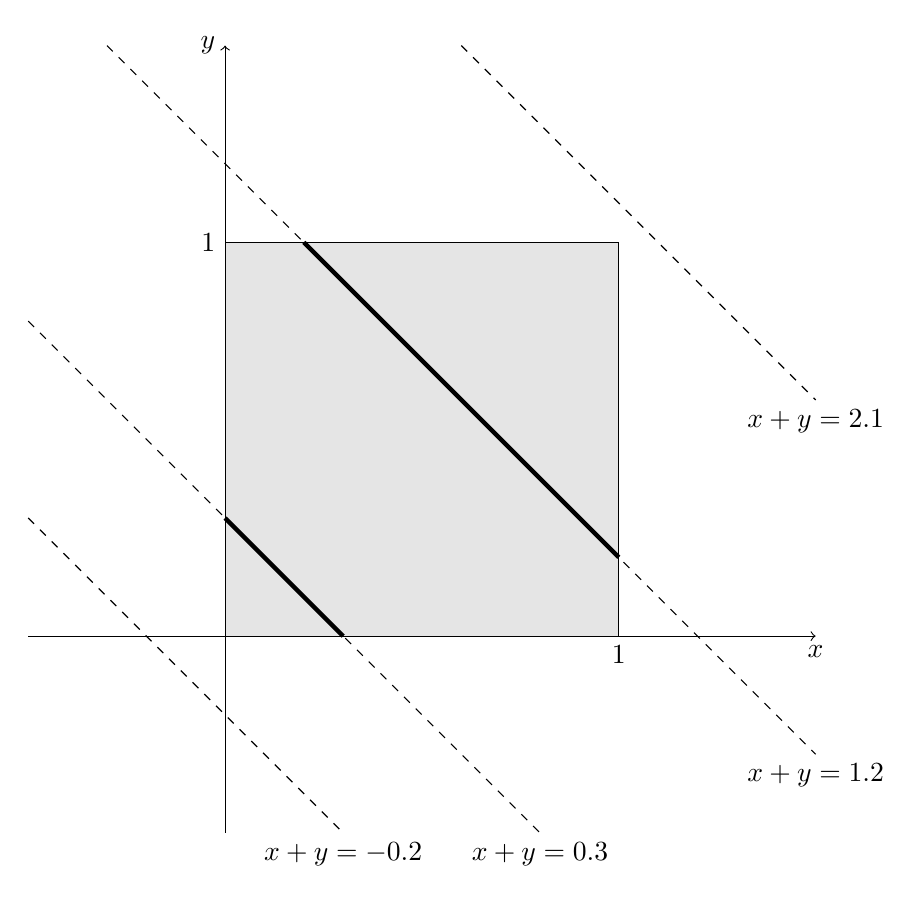
\begin{tikzpicture}[scale=5]
            % оси
            \draw [->] ( -0.5, 0 ) -- ( 1.5, 0 ) node [below] at ( 1.5, 0 ) {$x$};
            \draw [->] ( 0, -0.5 ) -- ( 0, 1.5 ) node [left] at ( 0, 1.5 ) {$y$};

            % квадратик
            \draw [fill=gray!20] ( 0, 0 ) rectangle ( 1, 1 );
            \node [below] at ( 1, 0 ) {$1$};
            \node [left] at ( 0, 1 ) {$1$};

            % прямые
            \draw [dashed] ( -0.5, 0.3 ) -- ( 0.3, -0.5 ) node [below] at ( 0.3, -0.5 ) {$x + y = -0.2$};
            \draw [dashed] ( -0.5, 0.8 ) -- ( 0.8, -0.5 ) node [below] at ( 0.8, -0.5 ) {$x + y = 0.3$};
            \draw [dashed] ( -0.3, 1.5 ) -- ( 1.5, -0.3 ) node [below] at ( 1.5, -0.3 ) {$x + y = 1.2$};
            \draw [dashed] ( 0.6, 1.5 ) -- ( 1.5, 0.6 ) node [below] at ( 1.5, 0.6 ) {$x + y = 2.1$};

            % отрезки
            \draw [ultra thick] ( 0, 0.3 ) -- ( 0.3, 0 );
            \draw [ultra thick] ( 0.2, 1 ) -- ( 1, 0.2 );
        \end{tikzpicture}
        \caption{Вычисление $f_Z(z)$: отрезки с ненулевыми значениями плотности.}
    \end{figure}

    Интеграл для второго случая ($0 < z \le 1$):
    \begin{equation}
        \int \limits_0^z f_{X,Y}(x,z-x) dx
        = \int \limits_0^z \left ( x + z - x \right ) dx
        = \int \limits_0^z z dx
        = \left . z x \right |_0^z
        = z^2
    \end{equation}

    Интеграл для третьего случая ($1 < z \le 2$):
    \begin{equation}
        \int \limits_{z-1}^1 f_{X,Y}(x,z-x) dx
        = \int \limits_{z-1}^1 \left ( x + z - x \right ) dx
        = \int \limits_{z-1}^1 z dx
        = \left . z x \right |_{z-1}^1
        = z - z (z - 1)
        = 2 z - z^2
    \end{equation}

    Таким образом,
    \begin{equation}
        f_Z(z)
        = \left \{
        \begin{array}{ll}
            0,        & z < 0       \\
            z^2,      & 0 < z \le 1 \\
            2z - z^2, & 1 < z \le 2 \\
            0,        & 2 < z
        \end{array}
        \right .
    \end{equation}

    \item Для величины $U$ сперва найдем функцию распределения:
    \begin{equation}
        F_U(u)
        = \probability{XY < u}
        = \left \{
        \begin{array}{ll}
            0,                                          & u < 0         \\
            \iint \limits_{xy < u} f_{X,Y}(x, y) dy dx, & 0 \le u \le 1 \\
            1,                                          & 1 < u
        \end{array}
        \right .
    \end{equation}

    Вычислим интеграл для второго случая ($0 \le u \le 1$):
    \begin{multline}
        \iint \limits_{xy < u} f_{X,Y}(x, y) dy dx
        = \int \limits_0^u \int \limits_0^1 ( x + y ) dy dx + \int \limits_u^1 \int \limits_0^{\frac{u}{x}} ( x + y ) dy dx = \\
        %
        = \int \limits_0^u \left . \left ( x y + \frac{y^2}{2} \right ) \right |_0^1 dx + \int \limits_u^1 \left . \left ( x y + \frac{y^2}{2} \right ) \right |_0^{\frac{u}{x}} dx = \\
        = \int \limits_0^u \left ( x + \frac{1}{2} \right ) dx + \int \limits_u^1 \left ( x \frac{u}{x} + \frac{u^2}{2x^2} \right ) dx = \\
        = \left . \left ( \frac{x^2}{2} + \frac{1}{2} x \right ) \right |_0^u + \left . \left ( u x + \frac{u^2}{2} \left ( - \frac{1}{x} \right ) \right ) \right |_u^1 dx = \\
        %
        = \frac{u^2}{2} + \frac{1}{2} u + u - \frac{u^2}{2} - u^2 - \frac{u^2}{2} \left ( - \frac{1}{u} \right )
        = \frac{1}{2} u + u - u^2 + \frac{u}{2}
        = 2 u - u^2
    \end{multline}

    \begin{figure}[!h]
        \center
        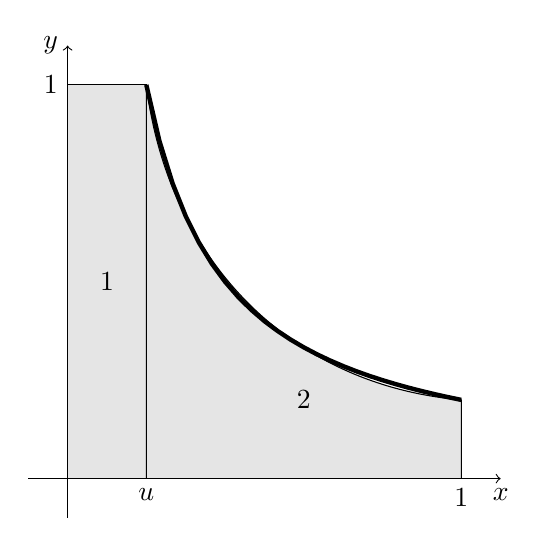
\begin{tikzpicture}[scale=5]
            % область 1
            \draw [fill=gray!20] ( 0, 0 ) rectangle ( 0.2, 1 );
            % область 2
            \draw [fill=gray!20] ( 0.2, 0 ) -- ( 0.2, 1 ) to [out=-83,in=175] ( 1, 0.2 ) -- ( 1, 0 );

            % оси
            \draw [->] ( -0.1, 0 ) -- ( 1.1, 0 ) node [below] at ( 1.1, 0 ) {$x$};
            \draw [->] ( 0, -0.1 ) -- ( 0, 1.1 ) node [left] at ( 0, 1.1 ) {$y$};

            % квадратик
            \node [below] at ( 1, 0 ) {$1$};
            \node [left] at ( 0, 1 ) {$1$};

            % гипербола
            \draw [ultra thick, domain=0.2:1] plot (\x, {0.2/\x});

            % пунктир
            \draw [dashed] ( 0.2, 0 ) -- ( 0.2, 1 ) node [below] at ( 0.2, 0 ) {$u$};

            % площади
            \node at ( 0.1, 0.5 ) {$1$};
            \node at ( 0.6, 0.2 ) {$2$};
        \end{tikzpicture}
        \caption{Вычисление $F_U(u)$: 1 - область первого интеграла, 2 - область второго интеграла.}
    \end{figure}

    Таким образом, функция распределения имеет вид:
    \begin{equation}
        F_U(u)
        = \left \{
        \begin{array}{ll}
            0,         & u < 0         \\
            2 u - u^2, & 0 \le u \le 1 \\
            1,         & 1 < u
        \end{array}
        \right .
    \end{equation}

    Откуда плотность вероятности $f_U(u)$ величины $U$:
    \begin{equation}
        f_U(u)
        = \derivative{u} F_U(u)
        = \left \{
        \begin{array}{ll}
            0,      & u < 0         \\
            2 - 2u, & 0 \le u \le 1 \\
            1,      & 1 < u
        \end{array}
        \right .
    \end{equation}

%        \item Плотность вероятности $f_U(u)$ величины $U$ найдем аналогичным образом:
%        \begin{equation}
%            f_U(u)
%            = \int \limits_{-\infty}^{\infty} f_{X,Y} \left ( x, \frac{u}{x} \right ) dx
%            = \left \{
%            \begin{array}{ll}
%                0,                                                              & u \le 0     \\
%                \int \limits_{u}^{1} f_{X,Y} \left ( x, \frac{u}{x} \right ) dx & 0 < u \le 1 \\
%                0,                                                              & 1 < u
%            \end{array}
%            \right .
%        \end{equation}
%
%        Интеграл во втором случае ($0 \le u \le 1$):
%        \begin{multline}
%            \int \limits_{u}^{1} f_{X,Y} \left ( x, \frac{u}{x} \right ) dx
%            = \int \limits_{u}^{1} \left ( x + \frac{u}{x} \right ) dx
%            = \left . \left ( \frac{x^2}{2} + u \ln x \right ) \right |_u^1 = \\
%            %
%            = \frac{1}{2} + u \ln 1 - \frac{u^2}{2} - u \ln u
%            = \frac{1}{2} - \frac{u^2}{2} - u \ln u
%        \end{multline}
\end{enumerate}

\subsection*{Ответ:}
\begin{enumerate}
    \item Плотность вероятности величины $Z$:
    $$
    f_Z(z)
    = \left \{
    \begin{array}{ll}
        0,        & z < 0       \\
        z^2,      & 0 < z \le 1 \\
        2z - z^2, & 1 < z \le 2 \\
        0,        & 2 < z
    \end{array}
    \right .
    .
    $$

    \item Плотность вероятности величины $U$:
    $$
    f_U(u)
    = \derivative{u} F_U(u)
    = \left \{
    \begin{array}{ll}
        0,      & u < 0         \\
        2 - 2u, & 0 \le u \le 1 \\
        1,      & 1 < u
    \end{array}
    \right .
    .
    $$
\end{enumerate}


\section*{Задача 18.521}

Случайные величины $X$ и $Y$ независимы и одинаково распределены по закону $\mathcal{N}(0, \sigma^2)$. Установить, по какому закону распределена случайная величина
$R = \sqrt{X^2 + Y^2}$.
\subsection*{Решение:}
Пусть $F_R(r)$ --- функция распределения величины $R$:
\begin{multline}
    F_R(r)
    = \probability{R < r}
    = \probability{\sqrt{X^2 + Y^2} < r}
    = \probability{X^2 + Y^2 < r^2} = \\
    %
    = \left \{
    \begin{array}{ll}
        0,                                                   & r \le 0 \\
        \iint \limits_{x^2 + y^2 < r^2} f_{X,Y}(x, y) dy dx, & 0 < r   \\
    \end{array}
    \right .
\end{multline}
где $f_{X,Y}(x, y)$ --- совместная плотность вероятности вектора $\left ( X, Y \right )$, равная произведению плотности вероятности $f_X(x)$ величины $X$ и
плотности вероятности $f_Y(y)$ величины $Y$ поскольку величины $X$ и $Y$ \textbf{независимы}:
\begin{equation}
    f_{X,Y}(x, y) = f_X(x) \cdot f_Y(y),
\end{equation}
Одномерные плотности имеют одинаковый вид:
\begin{gather}
    f_X(x) = \frac{1}{\sqrt{2 \pi} \sigma} e^{- \frac{x^2}{2 \sigma^2}} , \\
    f_Y(y) = \frac{1}{\sqrt{2 \pi} \sigma} e^{- \frac{y^2}{2 \sigma^2}} .
\end{gather}

Вычислим итеграл в функции распределения (случай $0 < r$):
\begin{equation}
    \iint \limits_{x^2 + y^2 < r^2} f_{X,Y}(x, y) dy dx
    = \iint \limits_{x^2 + y^2 < r^2} \frac{1}{\sqrt{2 \pi} \sigma} e^{- \frac{x^2}{2 \sigma^2}} \cdot \frac{1}{\sqrt{2 \pi} \sigma} e^{- \frac{y^2}{2 \sigma^2}} dy dx
    = \iint \limits_{x^2 + y^2 < r^2} \frac{1}{2 \pi \sigma^2} e^{- \frac{x^2 + y^2}{2 \sigma^2}} dy dx
\end{equation}
Для вычисления итеграла перейдем к полярным координатам
\begin{gather}
    x = \rho \cos \varphi , \\
    y = \rho \sin \varphi .
\end{gather}
Якобиан преобразования:
\begin{equation}
    J
    = \begin{vmatrix}
          \cos \varphi & - \rho \sin \varphi \\
          \sin \varphi & \rho \cos \varphi   \\
    \end{vmatrix}
    = \rho \cos^2 \varphi + \rho \sin^2 \varphi = \rho
    .
\end{equation}

В результате замены интеграл принимает вид
\begin{multline}
    \iint \limits_{x^2 + y^2 < r^2} f_{X,Y}(x, y) dy dx
    = \iint \limits_{\rho^2 < r^2, 0 \le \varphi \le 2 \pi} \frac{1}{2 \pi \sigma^2} e^{- \frac{\rho^2}{2 \sigma^2}} \rho d \varphi d \rho
    = \int \limits_0^{r} \int \limits_0^{2 \pi} \frac{1}{2 \pi \sigma^2} e^{- \frac{\rho^2}{2 \sigma^2}} \rho d \varphi d \rho = \\
    %
    = \int \limits_0^{r} 2 \pi \frac{1}{2 \pi \sigma^2} e^{- \frac{\rho^2}{2 \sigma^2}} \rho d \rho
    = \int \limits_0^{r} \frac{\rho}{\sigma^2} e^{- \frac{\rho^2}{2 \sigma^2}} d \rho
    = \left . \left ( - e^{- \frac{\rho^2}{2 \sigma^2}} \right ) \right |_0^{r}
    = 1 - e^{-\frac{r^2}{2 \sigma^2}}
\end{multline}

Таким образом, функция распределения величины $R$:
\begin{equation}
    F_R(r)
    = \left \{
    \begin{array}{ll}
        0,                               & r \le 0 \\
        1 - e^{-\frac{r^2}{2 \sigma^2}}, & 0 < r   \\
    \end{array}
    \right .
\end{equation}
и плотность вероятности величины $R$:
\begin{equation}
    f_R(r)
    = \derivative{r} F_R(r)
    = \left \{
    \begin{array}{ll}
        0,                                                                       & r \le 0 \\
        - e^{-\frac{r^2}{2 \sigma^2}} \left ( - \frac{2 r}{2 \sigma^2} \right ), & 0 < r   \\
    \end{array}
    \right .
    = \left \{
    \begin{array}{ll}
        0,                                              & r \le 0 \\
        \frac{r}{\sigma^2} e^{-\frac{r^2}{2 \sigma^2}}, & 0 < r   \\
    \end{array}
    \right .
\end{equation}
\subsection*{Ответ:}
Закон распределения Релея. Функция плотности вероятности $f(r)$:
$$
f(r)
= \left \{
\begin{array}{ll}
    0,                                              & r \le 0 \\
    \frac{r}{\sigma^2} e^{-\frac{r^2}{2 \sigma^2}}, & 0 < r   \\
\end{array}
\right .
$$

\section*{Задачи для самостоятельного решения}

Из раздела 18 сборника задач Ефимова и Поспелова.
\begin{enumerate}
    \item На занятии: 445, 459.
    \item Дома: 378 -- 381, 389, 393, 411 -- 413, 423, 431.
\end{enumerate}

Из сборника задач типового расчёта Чудесенко: 30.

Задачи 514, 517, 518.

Задачи 436, 437, 439, 441, 444.
